\documentclass[11pt, a4paper]{article}
\usepackage[utf8]{inputenc}
\usepackage[margin=1in]{geometry} %Sets proper 1-inch margins. 
\usepackage{amsmath} %Only load this if you are using math/equations.
\usepackage{graphicx} %Only need to call this if inserting images.
\usepackage{caption} %Only need to call this if inserting captions.
\usepackage{float} %Allows the use of the [H] specifier. 
\graphicspath{{../../assets/final_plots/}} %Sets the working directory for images.
\usepackage[colorlinks,citecolor=blue,linkcolor=blue,urlcolor=blue]{hyperref} %Allows for the embedding of urls. 
\usepackage{listings}
\lstset{%
   breaklines=true
}

\usepackage{natbib}
\usepackage{longtable}
\usepackage{lscape}
\usepackage{blindtext}
\usepackage{xcolor}
\usepackage{rotating}
\usepackage{tabularx}
\usepackage{booktabs}

\newcommand{\comment}[1]{}

\usepackage{fancyhdr}
\pagestyle{fancy}
\fancyhf{}
\rhead{Jonah Edmundson}
\lhead{\thepage}

\begin{document}
\begin{center}
\textsc{A Report} \par
\small{\textsc{For the}} \par
\Large{\textsc{SEGMENTATION OF STATISTICS CANADA’S PROXIMITY MEASURES}}
\par
\vspace{0.917 pc} %Creates a paragraph line break. 
\par
\normalsize{ }

\thispagestyle{empty}

\vspace{8 pc} %Creates a paragraph line break. 


\par
June 2023	
\par
\vspace{8pc}

Ricky Heinrich \par
Noman Mohammad \par
Avishek Saha \par 
Jonah Edmundson


%\vspace{0.917 pc} %Creates a paragraph line break. 
%\vspace{0.917 pc} %Creates a paragraph line break. 
\par
\vfill
\thispagestyle{empty}
\par
\noindent\small{Statistics Canada Liaison - Jérôme Blanchet, Bjenk Ellefsen}
\par
\noindent\small{UBCO Project Supervisor - His Excellency Dr. Firas Moosvi}
\par
\vspace{2pc}
\par
\noindent\tiny{In compliance with the Capstone Project requirements of the MDS program at the University of British Columbia - Okanagan.}
\end{center}
\normalsize

\pagebreak



\thispagestyle{empty}
\tableofcontents
\thispagestyle{empty}

\pagebreak
\thispagestyle{empty}
\listoffigures
\thispagestyle{empty}

\vspace{2pc}

\pagebreak
\thispagestyle{empty}
%\small{\listoftables}
\listoftables
\pagebreak


%%%%%%%%%%%%%%%%%%%%%%%%%%%%%%%%%%%%%%%%
\section{Introduction}
%%%%%%%%%%%%%%%%%%%%%%%%%%%%%%%%%%%%%%%%
\par

\setcounter{page}{1}

\normalsize
The

















\pagebreak 
%%%%%%%%%%%%%%%%%%%%%%%%%%%%%%%%%%%%%%%%
\section{Background}
%%%%%%%%%%%%%%%%%%%%%%%%%%%%%%%%%%%%%%%%






















\pagebreak 
%%%%%%%%%%%%%%%%%%%%%%%%%%%%%%%%%%%%%%%%
\section{Data}
%%%%%%%%%%%%%%%%%%%%%%%%%%%%%%%%%%%%%%%%


text




\subsection{Primary Dataset}


















\subsection{Missing Values}










\begin{table}[H]
\centering
%\caption{caption goes here}\label{table1}
\begin{tabular}{|l|l|} 
\hline
\textbf{Symbol} & \textbf{Meaning} \\
\hline
. & not available for any reference period \\ 
\hline 
.. & not available for a specific reference period \\ 
\hline 
... & not applicable \\ 
\hline 
F & too unreliable to be published \\ 
\hline 
\end{tabular}
\end{table}






% latex table generated in R 3.6.3 by xtable 1.8-4 package
% Tue May 30 13:11:59 2023
\begin{table}[ht]
\centering
\begin{tabular}{rcc}
  \hline
 & DBs with Data Available & Percentage \\ 
  \hline
Employment & 423,602 & 86.5 \\ 
  Pharmacy & 178,521 & 36.5 \\ 
  Childcare & 243,964 & 49.8 \\ 
  Healthcare & 300,465 & 61.4 \\ 
  Grocery & 141,063 & 28.8 \\ 
  Pri. Educ. & 225,359 & 46.0 \\ 
  Sec. Educ. & 141,213 & 28.8 \\ 
  Library & 112,655 & 23.0 \\ 
  Parks & 234,068 & 47.8 \\ 
  Transit & 181,305 & 37.0 \\ 
  DB Pop. & 487,526 & 99.6 \\ 
   \hline
\end{tabular}
\end{table}








\subsection{Other Data}
























\pagebreak 
%%%%%%%%%%%%%%%%%%%%%%%%%%%%%%%%%%%%%%%%
\section{Methods}
%%%%%%%%%%%%%%%%%%%%%%%%%%%%%%%%%%%%%%%%



text






\subsection{Data Exploration}
















\subsection{Clustering Tendency}













\subsection{Quintiles}













\subsection{Minima Identification}











\subsection{Clustering}








\subsubsection{Number of Clusters}











\subsubsection{Comparison of Algorithms}










\subsubsection{Cluster Profiles}























\pagebreak 
%%%%%%%%%%%%%%%%%%%%%%%%%%%%%%%%%%%%%%%%
\section{Results}
%%%%%%%%%%%%%%%%%%%%%%%%%%%%%%%%%%%%%%%%


text







\subsection{Data Exploration}

\subsubsection{Summary Statistics}








% latex table generated in R 3.6.3 by xtable 1.8-4 package
% Sat Jun 10 08:13:30 2023
\begin{sidewaystable}[ht]
\centering
\begin{tabular}{rlllllllllll}
  \hline
 & Employment & Pharmacy & Childcare & Healthcare & Grocery & Pri. Educ. & Sec. Educ. & Library & Parks & Transit & DB Pop. \\ 
  \hline
1 Dec. & 1e-04 & 0.0075 & 0.0079 & 2e-04 & 0.0144 & 0.0319 & 0.0374 & 0.0508 & 0.0127 & 0.0011 & 0 \\ 
  2 Dec. & 4e-04 & 0.0098 & 0.0152 & 7e-04 & 0.0221 & 0.0416 & 0.0421 & 0.0558 & 0.0203 & 0.0026 & 0 \\ 
  3 Dec. & 0.0013 & 0.0146 & 0.0241 & 0.0018 & 0.0289 & 0.0582 & 0.0485 & 0.0624 & 0.0278 & 0.0045 & 5 \\ 
  4 Dec. & 0.003 & 0.0193 & 0.0348 & 0.0032 & 0.0348 & 0.072 & 0.0586 & 0.0707 & 0.0372 & 0.0067 & 16 \\ 
  5 Dec. & 0.0065 & 0.0256 & 0.0476 & 0.005 & 0.0434 & 0.09 & 0.0745 & 0.0814 & 0.0481 & 0.0094 & 29 \\ 
  6 Dec. & 0.0127 & 0.0341 & 0.0636 & 0.0074 & 0.0555 & 0.1105 & 0.091 & 0.096 & 0.0614 & 0.0131 & 45 \\ 
  7 Dec. & 0.0217 & 0.0457 & 0.0846 & 0.0111 & 0.0719 & 0.1366 & 0.1141 & 0.1168 & 0.0793 & 0.0184 & 66 \\ 
  8 Dec. & 0.0368 & 0.0641 & 0.1167 & 0.0184 & 0.0985 & 0.172 & 0.1492 & 0.1488 & 0.105 & 0.0272 & 100 \\ 
  9 Dec. & 0.0726 & 0.0983 & 0.1751 & 0.0343 & 0.154 & 0.233 & 0.2128 & 0.2106 & 0.1494 & 0.0442 & 173 \\ 
  Min. & 0 & 0 & 0 & 0 & 1e-04 & 4e-04 & 5e-04 & 1e-04 & 0 & 0 & 0 \\ 
  Median & 0.0065 & 0.0256 & 0.0476 & 0.005 & 0.0434 & 0.09 & 0.0745 & 0.0814 & 0.0481 & 0.0094 & 29 \\ 
  Mean & 0.02541 & 0.04438 & 0.07584 & 0.01372 & 0.06991 & 0.11617 & 0.104 & 0.11462 & 0.0692 & 0.01805 & 72 \\ 
  Max. & 1 & 1 & 1 & 1 & 1 & 1 & 1 & 1 & 1 & 1 & 7607 \\ 
  Std. Dev. & 0.0491 & 0.0579 & 0.0874 & 0.0279 & 0.0783 & 0.0917 & 0.0869 & 0.0978 & 0.0685 & 0.027 & 146 \\ 
  Skew & 4.656 & 4.555 & 2.807 & 7.041 & 3.201 & 1.963 & 2.462 & 3.439 & 2.824 & 5.692 & 8 \\ 
  Kurtosis & 38.08 & 37.81 & 14.82 & 95.45 & 17.83 & 8.72 & 11.84 & 18.48 & 17.2 & 72.96 & 152 \\ 
   \hline
\end{tabular}
\end{sidewaystable}










%%%%%%%%%%%%
\begin{longtable}{|l|c|}
\hline
\textbf{Variable}  & \textbf{Counts}  \\
\hline
{DBs Per Province} &  \\
\indent\indent \textit{Alberta} & 66,749 \\
\indent\indent \textit{British Columbia} & 52,850 \\
\indent\indent \textit{Manitoba} & 30,669 \\
\indent\indent \textit{New Brunswick} & 14,345 \\
\indent\indent \textit{Newfoundland and Labrador} & 8,756 \\
\indent\indent \textit{Northwest Territories} & 1,495 \\
\indent\indent \textit{Nova Scotia} & 15,279 \\
\indent\indent \textit{Nunavut} & 792 \\
\indent\indent \textit{Ontario} & 133,214 \\
\indent\indent \textit{Prince Edward Island} & 3,639 \\
\indent\indent \textit{Quebec} &  106,251 \\
\indent\indent \textit{Saskatchewan} & 54,118 \\
\indent\indent \textit{Yukon} & 1,519 \\
\hline

{CMA Type} &  \\
\indent\indent \textit{CMA (B)} & 206,709 \\
\indent\indent \textit{Untracted CA (D)} & 53,061 \\
\indent\indent \textit{Tracted CA (K)} & 16,992 \\
\indent\indent \textit{Not a CMA or CA} & 212,914 \\
\hline

{Amenity Dense} &  \\
\indent\indent \textit{Low Density (0)} & 442,179 \\
\indent\indent \textit{Medium Density (1)} & 37,303 \\
\indent\indent \textit{High Density (2)} & 4,827 \\
\indent\indent \textit{Too unreliable to publish (F)} & 5,367 \\
\hline

{Suppressed} &  \\
\indent\indent \textit{Not suppressed (0)} & 484,309 \\
\indent\indent \textit{Info. Suppressed (1)} & 5,367 \\
\hline

\hline
\end{longtable}







\subsubsection{Distributions}

example text Figure~\ref{comparedist} ...




\begin{figure}[H]
\centering
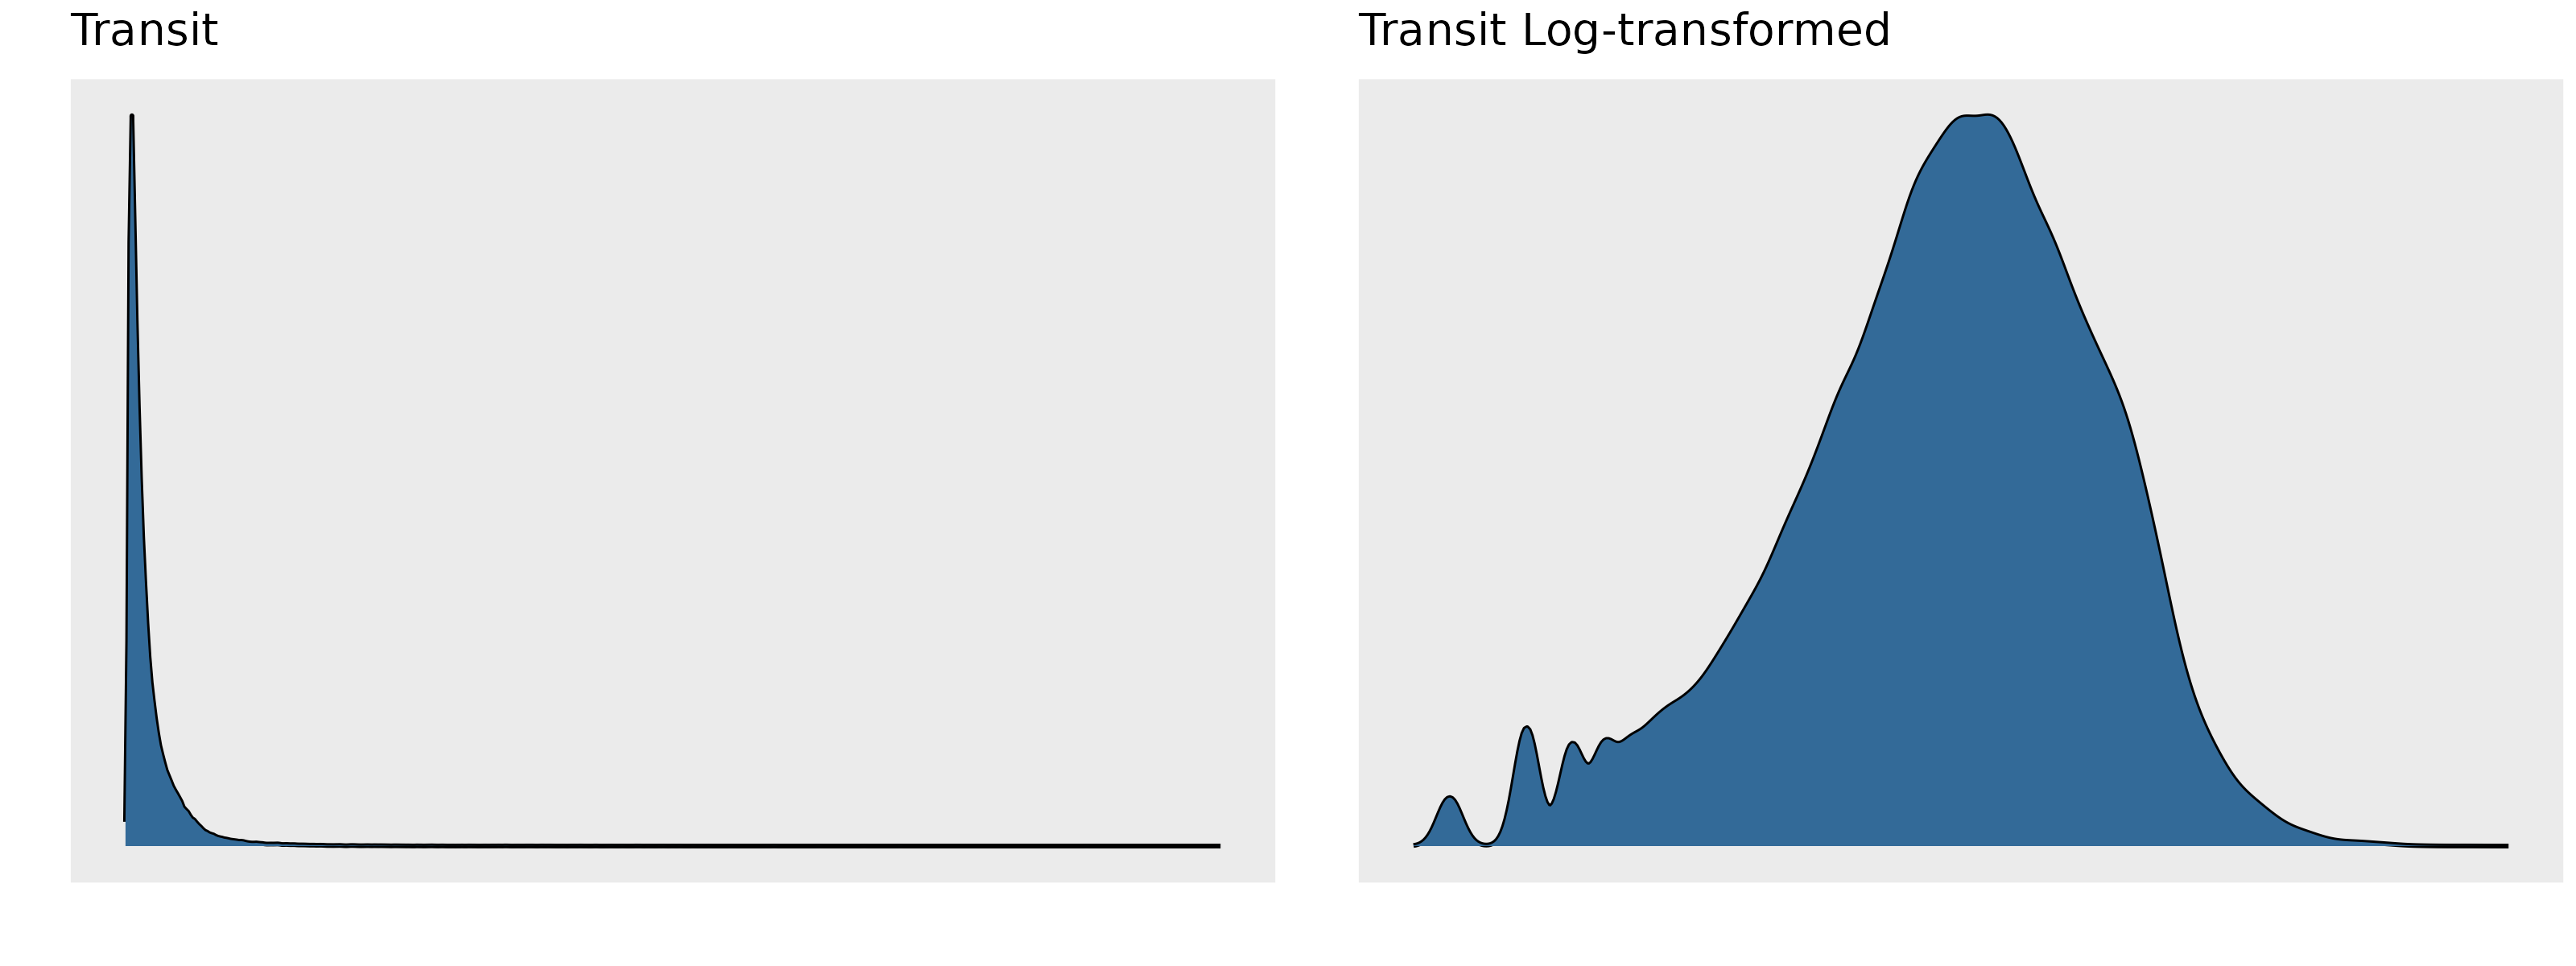
\includegraphics[scale=0.8]{./distributions/compare_distributions.png}
\caption[Comparison of distributions]{Distribution of the proximity measure to primary education services before and after log-transformation.}\label{comparedist}
\end{figure}






% latex table generated in R 3.6.3 by xtable 1.8-4 package
% Wed May 31 09:55:20 2023
\begin{table}[h]
\centering
\begin{tabular}{rllll}
  \hline
 & Counts & Percentages & Log Transformed Counts & Log Transformed Percentages \\ 
  \hline
Employment & 45,390 & 9.27 & 0 & 0.00 \\ 
  Pharmacy & 13,416 & 2.74 & 478 & 0.10 \\ 
  Childcare & 15,397 & 3.14 & 140 & 0.03 \\ 
  Healthcare & 31,007 & 6.33 & 50 & 0.01 \\ 
  Grocery & 11,904 & 2.43 & 794 & 0.16 \\ 
  Pri. Educ. & 10,205 & 2.08 & 98 & 0.02 \\ 
  Sec. Educ. & 8,683 & 1.77 & 215 & 0.04 \\ 
  Library & 8,867 & 1.81 & 2,295 & 0.47 \\ 
  Parks & 12,703 & 2.59 & 910 & 0.19 \\ 
  Transit & 14,165 & 2.89 & 3,596 & 0.73 \\ 
   \hline
\end{tabular}
\end{table}














\subsection{Clustering Tendency}













\subsection{Quintiles}













\subsection{Minima Identification}











\subsection{Clustering}













\subsubsection{Cluster Profiles}










\pagebreak 
%%%%%%%%%%%%%%%%%%%%%%%%%%%%%%%%%%%%%%%%
\section{Discussion}
%%%%%%%%%%%%%%%%%%%%%%%%%%%%%%%%%%%%%%%%




text 







\subsection{Comparison of Approaches}


















\subsection{Interpretation of Cluster Profiles}
























\pagebreak 
%%%%%%%%%%%%%%%%%%%%%%%%%%%%%%%%%%%%%%%%
\section{Limitations}
%%%%%%%%%%%%%%%%%%%%%%%%%%%%%%%%%%%%%%%%

























\pagebreak 
%%%%%%%%%%%%%%%%%%%%%%%%%%%%%%%%%%%%%%%%
\section{Conclusion}
%%%%%%%%%%%%%%%%%%%%%%%%%%%%%%%%%%%%%%%%


\subsection{Successful Methods}











\subsection{Unsuccessful Methods}

\subsubsection{Univariate Clustering}









\subsubsection{Multivariate Clustering}










\subsection{Extra Plots and Tables}





































\pagebreak
\section{References}


\bibliographystyle{apa}
\renewcommand{\bibsection}{}
\bibliography{final_sources.bib}



\pagebreak
\appendix
\section{Appendix}
\par
text








\end{document}
